\chapter{Evaluación y resultados}\label{cap:resultados}\label{cap:experimentos}

Con los dieciséis algoritmos ya formulados en la Sección~\ref{cap:algoritmos}, este capítulo los somete al protocolo de evaluación
offline, con las métricas definidas en la Sección~\ref{sec:arte-fundamentos}, y presenta los
resultados publicados junto con una discusión honesta de lo que permiten y de lo que no
permiten concluir. El énfasis no está en declarar un ganador, sino en dejar trazable cada cifra
hasta el corpus, la semilla, el reparto y la configuración exactos que la produjeron.

La evaluación se ejecuta sobre la misma plataforma descrita en los capítulos anteriores: los
usuarios sintéticos, sus bibliotecas y el corpus gobernado viven en la misma base de datos que
sirve la aplicación.

\section{Protocolo de evaluación}\label{sec:exp-protocolo}

La evaluación publicada se ejecutó offline con el corpus congelado \texttt{2026.09.2}. La población experimental contiene 400 usuarios sintéticos activos, generados de forma determinista; 79 cumplen la elegibilidad del split de prueba. Los perfiles se generan a partir de arquetipos (monogénero severo y generoso, omnívoro medio, completista de saga, explorador de novedades, coleccionista de pendientes, jugador ocasional con arranque en frío y veterano de biblioteca grande) que varían el número de géneros preferidos, el tamaño de la biblioteca, la generosidad al puntuar y la mezcla de estados, y llevan el marcador \texttt{synthetic-eval-user} para no contaminar el baseline de popularidad de la aplicación. No se utilizaron usuarios reales. El protocolo v15 fija semilla, versiones, snapshots, hashes, candidatas y exclusiones antes de consumir el test. La semilla permite reproducir esta ejecución, pero no sustituye un estudio de sensibilidad con múltiples semillas.

El protocolo vigente, v15, usa \emph{leave-fraction-out} por usuario, no
\emph{leave-one-out}: retiene varios ítems relevantes por persona en lugar de uno solo. Una
obra relevante es una entrada terminada o valorada con al menos siete medios puntos, con un
piso adicional de calidad externa (valoración agregada de origen de al menos 70 puntos) sobre
las candidatas a retener. Para cada usuario, el runner localiza su etiqueta de contenido con
más peso en el perfil y retira de ella un \(\lceil 0{,}3\times\) tamaño del grupo de esa
etiqueta\(\rceil\) de obras, nunca menos de una, retrocediendo de una en una si la retirada
desplazara esa etiqueta del primer puesto del perfil restante. Cuando ese mecanismo no se
puede construir para un usuario (sin ninguna señal de etiqueta de contenido, o sin candidatas
que superen el piso de calidad), el runner recurre al \emph{leave-one-out} simple de un único
ítem en lugar de excluir a esa persona del estudio; solo queda fuera quien no tiene ningún
positivo elegible en absoluto. Sobre los setenta y nueve usuarios evaluables, este mecanismo
retuvo doscientos dos ítems en total, una media de 2{,}56 por usuario con un rango de uno a
cinco. Todos los algoritmos reciben el mismo manifiesto de candidatas; el diseño evita
\emph{leakage}: ningún ítem retenido participa en la construcción del perfil, mientras que su
presencia entre las candidatas permite medir si se recupera.

Se calcula \(K\in\{5,10,20\}\). Si \(R_u\) es el conjunto relevante retenido de un usuario y
\(L_u^K\) los primeros \(K\) ítems de su lista, \(Precision@K=|L_u^K\cap R_u|/K\) y
\(Recall@K=|L_u^K\cap R_u|/|R_u|\). Al retener varios ítems por usuario, \(Recall@K\) deja de
ser binario y se convierte en una fracción continua, lo que aporta más información por
comparación que el \emph{leave-one-out} de una sola versión anterior del protocolo. El nDCG
y el MAP, definidos en la Sección~\ref{sec:arte-fundamentos}, se calculan sobre la misma
lista. El protocolo también conserva diversidad
intra-lista, novedad, coberturas y concentración cuando el artefacto permite estimarlas.

\section{Evolución del protocolo: tres intentos, no uno}\label{sec:exp-evolucion}\label{sec:exp-v15-fidelidad}

El protocolo v15 descrito arriba no fue el primero que se congeló y se ejecutó hasta el final
contra el split de prueba. Lo precedieron dos intentos completos, v12 y v14, cada uno
ejecutado una sola vez sobre el mismo split de test, con sus propios resultados publicados y
conservados sin alterar. Repasarlos aquí no es un ejercicio de transparencia añadido: la forma
concreta del protocolo v15 (retención por fracción sobre una etiqueta propia de cada usuario,
piso de calidad externa, población con mínimo garantizado) es la respuesta directa a dos
problemas reales que esos dos intentos anteriores dejaron medidos, no una elección de diseño
arbitraria.

\textbf{El protocolo v12 (10 de septiembre de 2026)} fue el primer cálculo congelado hasta el final. Su
resultado no fue una comparación entre algoritmos, sino un hallazgo metodológico: el
setenta y cuatro por ciento de los setenta y tres usuarios evaluables de aquel split
(cincuenta y cuatro de setenta y tres) caía en un modo de \enquote{historial insuficiente} del
recomendador de contenido en cuanto el \emph{leave-one-out} retiraba su único positivo
elegible, porque la población sintética de entonces no garantizaba un mínimo de positivos
por biblioteca. En ese modo, las diez variantes de contenido y sus derivadas dejaban de usar
similitud de etiquetas y colapsaban a la misma ordenación por valoración y popularidad que ya
usaban los baselines, de modo que quince de los dieciséis algoritmos publicaron precisión,
recall, nDCG y MAP exactamente en cero. La prueba de Friedman fue significativa
(\(\chi^2=30{,}00\), \(p=0{,}0119\), \(n=73\)), pero ninguna de las ciento veinte
comparaciones por pares sobrevivió la corrección de Holm: bajo ese protocolo, ningún
algoritmo era declarable superior a otro. Se verificó que no era un fallo del código de
puntuación (los vectores de contenido coincidían byte a byte con la caché versionada y el
conjunto de candidatas era idéntico para los dieciséis algoritmos), sino una interacción entre
dos piezas congeladas por separado: el generador de población sintética y el umbral de
arranque en frío del recomendador de contenido.

Corregir esa interacción exigió dos cambios sucesivos. El primero, ya con población
rediseñada, amplió el tamaño de biblioteca sintética, ensanchó la franja de popularidad de
origen y garantizó un mínimo de cinco positivos elegibles por biblioteca, lo que eliminó por
completo el modo de historial insuficiente en el split de prueba: pasó de afectar al setenta y
cuatro por ciento de los usuarios a un cero por ciento. El segundo cambio añadió, sobre esa
población ya corregida, un piso de calidad externa (valoración agregada de origen de al menos
setenta puntos) al ítem que el \emph{leave-one-out} podía retirar, para que el positivo
retenido no dependiera solo del gusto personal simulado sino también de una señal de calidad
independiente, cerrando un sesgo de popularidad conocido en la literatura de evaluación de
recomendadores~\cite{cremonesi2010performance}.

\textbf{El protocolo v14 (11 de septiembre de 2026)}, con esos dos cambios ya aplicados, sí produjo un
ganador defendible: \texttt{hybrid-weighted-cf-v1} (\(nDCG@10=0{,}1526\)) y
\texttt{content-cbf-weighted-v1} (\(0{,}1452\)) superaron con significación a los baselines y
a \texttt{recency-v1}, con catorce de las ciento veinte comparaciones por pares significativas
tras Holm, frente a cero en v12 (\(\chi^2=105{,}28\), \(p=1{,}29\times10^{-15}\), \(n=79\)). La
diversidad intra-lista y la concentración de recomendaciones mejoraron en la misma medida: el
índice de concentración de Herfindahl-Hirschman pasó de un rango de 0,55 a 0,71 en v12, propio
de un catálogo minúsculo de recomendaciones repetidas, a un rango de 0,005 a 0,03, consecuencia
directa de que el contenido ya no colapsaba al mismo \emph{fallback} que los baselines. Aun
así, v14 seguía reteniendo un único ítem por usuario mediante \emph{leave-one-out}: cada
comparación por usuario solo podía acertar o fallar una vez, lo que limitaba cuántas
diferencias entre algoritmos podían alcanzar significación. El colaborativo puro, por ejemplo,
no llegó a diferenciarse de forma significativa de ningún otro algoritmo en v14, pese a tener
un nDCG@10 más bajo que las variantes de contenido con mejor combinación.

Ese límite de potencia estadística, no un defecto de v14, es lo que motivó el cambio final a
\emph{leave-fraction-out} por etiqueta dominante propia de cada usuario que define el
protocolo v15: retener varios positivos por persona en lugar de uno solo da a cada comparación
más información por usuario sin necesidad de una población mayor. El resultado, ya presentado
en la Sección~\ref{sec:exp-significacion}, fue el esperado: de catorce comparaciones
significativas en v14 a cincuenta y cuatro en v15, con una diferenciación entre contenido y
colaborativo puro que v12 y v14 no tenían potencia estadística suficiente para establecer.
Los tres protocolos y sus artefactos quedan versionados sin modificar: v15 no invalida ni
reescribe los resultados de v12 o v14, los sustituye como publicación vigente por haber
corregido, de forma medida y documentada, los problemas que los dos intentos anteriores dejaron
al descubierto.

Conviene defender por qué v15 se acerca más a una prueba realista de lo que los algoritmos
hacen, no simplemente a un protocolo ajustado para producir números más altos. La
justificación no es que v15 favorezca a ningún algoritmo concreto, sino que corrige tres
formas en las que v12 y v14 se apartaban de cómo se evalúa la recuperación en la literatura y
de cómo el propio sistema puntúa.

La primera es de encuadre metodológico. Retirar y comprobar la recuperación de un subconjunto
de valoraciones del historial de un usuario, en lugar de un único ítem, no es una invención de
este proyecto: es la generalización natural del esquema \emph{All-but-N}, ya nombrado así en
la literatura desde Breese, Heckerman y Kadie~\cite{breese1998empirical} y sistematizado por
Herlocker et al.~\cite{herlocker2004evaluating}, donde el \emph{leave-one-out} que usaban los
protocolos v6 a v14 es simplemente el caso particular \(N=1\). v15 no sale de ese marco: solo
deja de fijar \(N\) de forma global y lo calcula por usuario, en proporción al tamaño de su
propio grupo de obras con esa etiqueta.

La segunda es de fidelidad a la señal que el sistema realmente usa. \texttt{facet\_similarity()},
el código de puntuación que usan los dieciséis algoritmos tanto en la aplicación como en el
laboratorio, combina cada familia de faceta como una suma ponderada, nunca como una decisión
de un único rasgo ganador. Que la etiqueta retirada deje de ser la primera del perfil recalculado
del usuario, en el 21{,}3\,\% de los casos verificados antes de congelar el protocolo, no
convierte la prueba en menos válida: un perfil de contenido sigue apoyándose en esa etiqueta,
con menos peso relativo, exactamente igual que se apoyaría en cualquier otra bajo el mismo
mecanismo de puntuación~\cite{pazzani2007content}. Exigir que la etiqueta se mantuviera siempre
en primer lugar habría sido, de hecho, la elección menos fiel al propio sistema, porque
habría excluido usuarios reales para el algoritmo aunque no lo fueran para la prueba.

La tercera es de inclusión. Un usuario para el que el mecanismo por fracción no se puede
construir cae al \emph{leave-one-out} simple de los protocolos anteriores en lugar de quedar
fuera, lo que evita el sesgo de selección contrario, el de quedarse solo con los usuarios más
fáciles de evaluar y llamar a eso representativo.

Ninguno de los tres argumentos convierte v15 en evidencia sobre jugadores reales: sigue siendo
una evaluación sobre una población sintética y un corpus concretos, como recuerda la
Sección~\ref{sec:exp-amenazas}. Lo que sí establecen es que, dentro de esa simulación, v15
mide la pregunta que se propone medir (¿recupera el sistema contenido afín al gusto que la
propia biblioteca del usuario ya demuestra?) con más fidelidad al mecanismo de puntuación real
y con menos artefactos de diseño heredados que v12 o v14, no solo con mejores cifras.

\section{Resultados publicados}\label{sec:exp-resultados}\label{sec:exp-exito}

La Tabla~\ref{tab:resultados-ndcg10} resume \(nDCG@10\), MAP@10 y tiempo de pared de la cohorte \texttt{active\_history\_10\_to\_20} incluidos en el artefacto v15. Se muestra una tabla compacta para evitar repetir cuatro métricas por tres valores de \(K\); el artefacto versionado \texttt{evaluation-400-test-2026-09-12-v15.artifact.json} y su transcripción en \texttt{docs/verification/evaluation-cohorts-400-test-2026-09-12-v15.md} preservan la transcripción completa para \(K=5,10,20\).

\begin{table}[H]
\centering
\caption{Resultados v15 publicados para la cohorte indicada. No son resultados con usuarios reales.}\label{tab:resultados-ndcg10}
\small
\renewcommand{\arraystretch}{1.2}
\setlength{\tabcolsep}{3pt}
\begin{tabularx}{\textwidth}{@{}>{\ttfamily\raggedright\arraybackslash}p{0.41\textwidth}Y>{\raggedleft\arraybackslash}p{0.115\textwidth}>{\raggedleft\arraybackslash}p{0.115\textwidth}@{}}
\textnormal{Algoritmo} & \textnormal{Familia} & \textnormal{\footnotesize nDCG@10} & \textnormal{\footnotesize MAP@10} \\
\hline
random-v1 & baseline & 0.00000 & 0.00000 \\
popularity-v1 & baseline & 0.00340 & 0.00098 \\
content-cbf-weighted-v1 & contenido & 0.17245 & 0.10878 \\
content-cbf-multiplicative-v1 & contenido & 0.08558 & 0.05934 \\
content-cbf-twostage-v1 & contenido & 0.11724 & 0.06767 \\
content-cbf-neg-v1 & contenido & 0.11778 & 0.07368 \\
content-cbf-weighted-pop-v1 & contenido + popularidad & 0.15181 & 0.09826 \\
content-cbf-multiplicative-pop-v1 & contenido + popularidad & 0.08517 & 0.05898 \\
content-cbf-twostage-pop-v1 & contenido + popularidad & 0.11410 & 0.06551 \\
content-cbf-neg-pop-v1 & contenido + popularidad & 0.09936 & 0.06134 \\
recency-v1 & contenido + novedad & 0.00594 & 0.00422 \\
content-cbf-mmr-v1 & contenido + diversidad & 0.13888 & 0.08685 \\
content-cbf-mmr-pop-v1 & contenido + diversidad & 0.13824 & 0.09353 \\
cf-user-knn-v1 & colaborativo & 0.02098 & 0.01099 \\
hybrid-weighted-cf-v1 & híbrido & 0.16989 & 0.10758 \\
hybrid-mmr-v1 & híbrido + diversidad & 0.15913 & 0.09741 \\
\end{tabularx}
\end{table}

La Tabla~\ref{tab:ndcg-todos-k} conserva \(nDCG\) en los tres cortes solicitados para el catálogo completo de variantes v15. Precision, recall y MAP permanecen en el artefacto y en la matriz de algoritmos para evitar una tabla de dieciséis filas y doce métricas que perdería legibilidad.

\begin{table}[H]
\centering
\caption{nDCG publicado por algoritmo y corte $K$ en v15.}\label{tab:ndcg-todos-k}
\tablecompact
\begin{tabularx}{\textwidth}{@{}>{\ttfamily\raggedright\arraybackslash}p{0.45\textwidth}Yrrr@{}}
\textnormal{Algoritmo} & \textnormal{Familia} & \textnormal{$K=5$} & \textnormal{$K=10$} & \textnormal{$K=20$} \\
\hline
random-v1 & baseline & 0.00000 & 0.00000 & 0.00000 \\
popularity-v1 & baseline & 0.00191 & 0.00340 & 0.00340 \\
content-cbf-weighted-v1 & contenido & 0.14114 & 0.17245 & 0.18987 \\
content-cbf-multiplicative-v1 & contenido & 0.07707 & 0.08558 & 0.10241 \\
content-cbf-twostage-v1 & contenido & 0.08827 & 0.11724 & 0.14002 \\
content-cbf-neg-v1 & contenido & 0.09656 & 0.11778 & 0.12992 \\
content-cbf-weighted-pop-v1 & contenido + popularidad & 0.13179 & 0.15181 & 0.17409 \\
content-cbf-multiplicative-pop-v1 & contenido + popularidad & 0.07677 & 0.08517 & 0.10200 \\
content-cbf-twostage-pop-v1 & contenido + popularidad & 0.08338 & 0.11410 & 0.14538 \\
content-cbf-neg-pop-v1 & contenido + popularidad & 0.08602 & 0.09936 & 0.11582 \\
recency-v1 & contenido + novedad & 0.00594 & 0.00594 & 0.00594 \\
content-cbf-mmr-v1 & contenido + diversidad & 0.11600 & 0.13888 & 0.16160 \\
content-cbf-mmr-pop-v1 & contenido + diversidad & 0.12211 & 0.13824 & 0.15362 \\
cf-user-knn-v1 & colaborativo & 0.01585 & 0.02098 & 0.03163 \\
hybrid-weighted-cf-v1 & híbrido & 0.14305 & 0.16989 & 0.18962 \\
hybrid-mmr-v1 & híbrido + diversidad & 0.13195 & 0.15913 & 0.17401 \\
\end{tabularx}
\end{table}

La diferencia numérica más visible en \(nDCG@10\) aparece entre \texttt{content-cbf-weighted-v1} y los baselines. El híbrido ponderado queda próximo a esa variante de contenido, mientras que el colaborativo aislado recupera menos positivos bajo este split. Esta observación es interna al artefacto: no prueba que contenido sea superior en una comunidad real, ni que los pesos del híbrido sean óptimos. De las tres variantes que publica la aplicación
(Sección~\ref{sec:alg-publicadas}), \texttt{content-cbf-weighted-v1} obtiene el mejor
\(nDCG@10\) (0.17245), \texttt{content-cbf-mmr-pop-v1} queda algo por debajo (0.13824) y
\texttt{recency-v1} apenas llega a 0.00594, lo que es coherente con su papel de variante de
descubrimiento, que prioriza la novedad sobre la afinidad. Para \(K=5\), \texttt{hybrid-weighted-cf-v1} publica \(nDCG=0.14305\), frente a \(0.14114\) de Weighted. Para \(K=20\), Weighted publica \(0.18987\) y el híbrido ponderado \(0.18962\). La proximidad de esas cifras ilustra por qué no basta con mirar la diferencia numérica sin contrastarla; la Sección~\ref{sec:exp-significacion} retoma esta misma comparación con una prueba estadística. El baseline aleatorio permanece en cero en la cohorte publicada; popularidad alcanza \(0.00340\) en \(nDCG@10\), lo que contextualiza la señal de contenido pero no mide utilidad subjetiva. La Figura~\ref{fig:ndcg-algoritmos} ordena los dieciséis algoritmos por \(nDCG@10\) y señala las tres variantes que publica la aplicación.

\begin{figure}[htp]
    \centering
    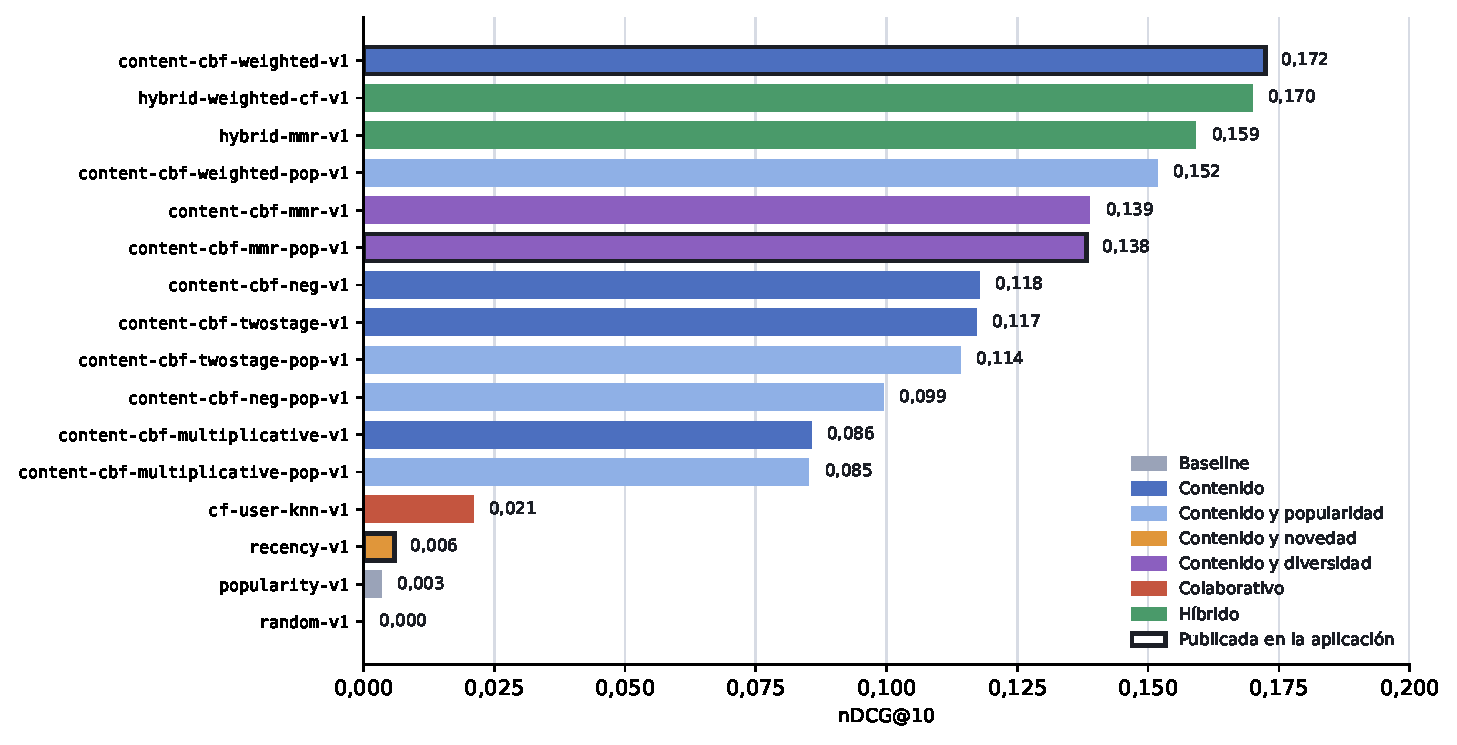
\includegraphics[width=0.9\textwidth]{figures/ndcg-algoritmos.pdf}
    \caption{\(nDCG@10\) de los dieciséis algoritmos en la evaluación v15, por familia. El borde grueso marca las tres variantes publicadas en la aplicación.}
    \label{fig:ndcg-algoritmos}
\end{figure}

nDCG y MAP resumen la recuperación en una única cifra por algoritmo, pero no responden
directamente a la pregunta más intuitiva: ¿a cuántas personas le funcionó? La
Tabla~\ref{tab:exito-usuarios} lo hace explícito para \(K=10\), sobre los doscientos dos
ítems retenidos y los setenta y nueve usuarios evaluables.

\begin{table}[H]
\centering
\caption{Éxitos por algoritmo a \(K=10\): ítems retenidos recuperados sobre 202; usuarios
que recuperaron al menos uno de los suyos sobre 79.}\label{tab:exito-usuarios}
\small
\begin{tabularx}{\textwidth}{@{}>{\ttfamily\raggedright\arraybackslash}X C{0.22\textwidth} C{0.25\textwidth}@{}}
\textnormal{Algoritmo} & \textnormal{Ítems@10 (/202)} & \textnormal{Usuarios\(\geq\)1@10 (/79)} \\
\hline
content-cbf-weighted-v1 & 48 & 39 (49\,\%) \\
hybrid-weighted-cf-v1 & 48 & 38 (48\,\%) \\
hybrid-mmr-v1 & 42 & 35 (44\,\%) \\
content-cbf-weighted-pop-v1 & 38 & 34 (43\,\%) \\
content-cbf-mmr-v1 & 36 & 32 (41\,\%) \\
content-cbf-neg-v1 & 34 & 28 (35\,\%) \\
cf-user-knn-v1 & 7 & 7 (9\,\%) \\
popularity-v1 & 2 & 2 (3\,\%) \\
recency-v1 & 1 & 1 (1\,\%) \\
random-v1 & 0 & 0 (0\,\%) \\
\end{tabularx}
\end{table}

Leída así, la mejor variante de contenido devuelve al menos uno de los juegos retenidos del
usuario, dentro de las diez primeras posiciones, casi a la mitad de las personas evaluables
(49\,\%), frente al 9\,\% del colaborativo puro y el 3\,\% o menos de los baselines; a
\(K=20\) esa cifra sube al 58\,\% para \texttt{content-cbf-weighted-v1} (cuarenta y seis de
setenta y nueve usuarios). Esta tasa de éxito por usuario y el \(nDCG@10\) de la
Tabla~\ref{tab:resultados-ndcg10} miden cosas distintas y no deben confundirse: la primera
cuenta aciertos binarios por persona, mientras que la segunda además descuenta la posición
exacta del acierto dentro de la lista, por lo que una tasa de éxito alta no implica un nDCG
igual de alto si los aciertos tienden a aparecer hacia el final del top-\(K\) en vez de al
principio.

\section{Significación estadística}\label{sec:exp-significacion}

Las diferencias de la Tabla~\ref{tab:resultados-ndcg10} se sometieron a contraste antes de
interpretarlas, con una cadena de pruebas pensada para el caso en que dieciséis algoritmos se
miden sobre exactamente los mismos setenta y nueve usuarios (medidas repetidas, no muestras
independientes) y se quiere comparar cada par sin inflar el número de falsos positivos que
salen solo por probar muchas comparaciones a la vez. La cadena tiene cuatro piezas, todas ellas
procedimientos estadísticos estándar aplicados a este problema concreto, no invenciones del
proyecto.

Primero, una prueba de \textbf{Friedman} sirve de ómnibus: comprueba, con un único contraste,
si existe alguna diferencia entre los dieciséis algoritmos antes de gastar el presupuesto de
comparaciones en mirar pares sueltos. Es no paramétrica (no asume que los valores de nDCG se
distribuyan de forma normal, algo que no se puede dar por hecho con solo setenta y nueve
observaciones) y adecuada para medidas repetidas: cada usuario aporta un ranking entre los
dieciséis algoritmos; la prueba contrasta si esos rankings son consistentes entre sí. Sobre
\(nDCG@10\), rechaza la hipótesis de igualdad con \(\chi^2=258{,}07\) y
\(p=2{,}69\times10^{-46}\).

Segundo, confirmada la existencia de alguna diferencia, cada uno de los ciento veinte pares
posibles de algoritmos se contrasta con una prueba de \textbf{Wilcoxon de rangos con signo
pareada}: para cada usuario se calcula la diferencia de \(nDCG@10\) entre los dos algoritmos
del par; la prueba comprueba si esas diferencias pareadas se alejan de cero de forma
consistente, sin asumir tampoco su distribución. Es la elección natural aquí porque los dos
algoritmos de cada par se miden sobre las mismas setenta y nueve personas, no sobre grupos
distintos.

Tercero, probar ciento veinte pares a la vez con un umbral \(p<0{,}05\) fijo produciría, solo
por azar, varios falsos positivos aunque ningún algoritmo fuera realmente distinto de otro
(el problema de comparaciones múltiples). La \textbf{corrección de Holm} ajusta el umbral de
significación de cada una de las ciento veinte comparaciones, ordenadas de menor a mayor \(p\)
sin corregir, de forma escalonada y más potente que una corrección de Bonferroni simple sin
dejar de controlar el error de tipo I acumulado. Cincuenta y cuatro de las ciento veinte
comparaciones siguen siendo significativas después de este ajuste.

Cuarto, además del contraste de hipótesis, el artefacto conserva un \textbf{intervalo de
confianza por \textit{bootstrap} BCa} (\emph{bias-corrected and accelerated}, dos mil
remuestreos, confianza del 95\,\%, semilla fija) para el \(nDCG@10\) de cada algoritmo, que da
un rango de valores plausibles en lugar de una única cifra puntual y no exige asumir ninguna
forma concreta para la distribución del estadístico. La Tabla~\ref{tab:significacion} recoge
las comparaciones por pares más relevantes para la narrativa de este capítulo; la lista
completa de las ciento veinte vive en el artefacto versionado.

\begin{table}[H]
\centering
\caption{Comparaciones por pares más relevantes sobre \(nDCG@10\), con corrección de Holm
sobre las ciento veinte comparaciones totales.}\label{tab:significacion}
\small
\begin{tabularx}{\textwidth}{@{}Yrr@{}}
\textnormal{Comparación} & \textnormal{\(\Delta\) nDCG@10} & \textnormal{\(p\) ajustado} \\
\hline
content-cbf-weighted-v1 vs.\ random-v1 & +0{,}1725 & 0{,}00001 \\
content-cbf-weighted-v1 vs.\ popularity-v1 & +0{,}1691 & 0{,}00001 \\
hybrid-weighted-cf-v1 vs.\ random-v1 & +0{,}1699 & 0{,}00001 \\
cf-user-knn-v1 vs.\ content-cbf-weighted-v1 & \(-\)0{,}1515 & 0{,}00004 \\
cf-user-knn-v1 vs.\ hybrid-weighted-cf-v1 & \(-\)0{,}1489 & 0{,}00004 \\
\end{tabularx}
\end{table}

Dos lecturas se derivan de este contraste. La primera es que tanto las variantes de contenido
como los híbridos superan a los dos baselines y a \texttt{recency-v1} con significación
sobrada, lo que sí permite descartar el azar como explicación de esas diferencias concretas,
bajo este corpus y esta población. La segunda, nueva en este protocolo frente a versiones
anteriores, es que el colaborativo puro (\texttt{cf-user-knn-v1}) resulta significativamente
peor que ocho de las diez variantes de contenido, una diferenciación que la potencia
estadística de protocolos previos no alcanzaba a establecer con esta claridad. Esa lectura
tiene un matiz importante: esta prueba mide específicamente la recuperación de obras de la
etiqueta de contenido dominante del perfil de cada usuario, y \texttt{cf-user-knn-v1} no usa
etiquetas en absoluto, sino similitud de patrones de valoración entre usuarios. La diferencia
es real y significativa, pero mide precisamente el terreno que la señal colaborativa no
modela; no es evidencia de que el filtrado colaborativo sea inferior en una tarea distinta,
como recuperar valoraciones de usuarios con gustos parecidos sin restricción de género. Los
híbridos combinan ambas señales en parte por esta razón: para no depender de ninguna de las
dos en solitario.

\section{Diversidad, cobertura y amenazas a la validez}\label{sec:exp-amenazas}

MMR introduce un objetivo distinto de la recuperación puntual: reducir redundancia entre elementos ya seleccionados. Sus resultados deben leerse junto con diversidad intra-lista, novedad, cobertura del catálogo, cobertura de predicción y HHI cuando el artefacto los publica. Una mejora de diversidad no compensa automáticamente una pérdida de nDCG, ni la métrica de acierto debe ocultar concentración. SavePoint mantiene estas medidas separadas para que el compromiso sea auditable.

Las amenazas principales son población sintética, un solo consumo del test y dependencia de
metadatos externos gobernados. El corpus y el snapshot son fortalezas de reproducibilidad,
pero acotan la generalización: la significación estadística de la Sección~\ref{sec:exp-significacion}
respalda que las diferencias observadas no son ruido bajo este corpus y esta población, no
que se sostengan sobre usuarios reales. Un estudio posterior debería incluir más semillas,
sensibilidades de hiperparámetros, datos observados con consentimiento y evaluación con
participantes, sin mutar el artefacto v15 ya publicado.

Este capítulo ha presentado la evaluación experimental de los algoritmos. El capítulo siguiente
cierra la memoria con el grado de cumplimiento de los objetivos y las líneas de continuación.
